\section{The image reconstruction problem of radio interferometers}
In Astronomy, one goal is to find ever smaller objects in the sky. For this purpose, we build instruments with higher angular resolution. The instruments angular resolution depends on two factors: On the diameter of the antenna-dish or mirror, and on the observed wavelength. With longer wavelengths we need bigger dishes/mirrors to achieve a similar angular resolution. 

This is an issue for Radio Astronomy. The long radio wavelengths require huge dishes for a high angular resolution. Of course there is a practical limit on the antenna-dish diameter we can build. The famous Arecibo observatory is one of the largest single-dish radio telescopes with a diameter of 305 meters. Antennas with such a large diameter become difficult to steer accurately, let alone the construction costs. We have reached the practical limits of single-dish telescopes. If we require higher angular resolution, we need to look at another type of instrument: The radio interferometer. They use several smaller antennas together, acting like a single large dish. An interferometer can achieve angular resolutions which are comparable to dishes with a diameter of several kilometers.

But there are drawbacks: The interferometer does not measure the sky in pixels. It measures the sky in Fourier space. As such, an interferometer produces amplitude and phase for each Fourier component that was measured. The observed image has to be reconstructed from the Fourier measurement. The measured Fourier components are called visibilities in the Radio Astronomy literature. From this point forward, we will call the measured Fourier components visibilities. The Figure \ref{intro0:inversefig} shows an example of the image reconstruction problem. The Figure \ref{intro0:inversefig:uvspace} shows the measurements in the Fourier space, and the figure \ref{intro0:inversefig:reconstruction} shows the observed image of the sky, with two stars close to each other. The image reconstruction has to find the observed image \ref{intro0:inversefig:reconstruction} from the measurements \ref{intro0:inversefig:uvspace}. 

\begin{figure}[htp]
	% preliminary
	\sbox\twosubbox{%
		\resizebox{\dimexpr.8\textwidth-1em}{!}{%
			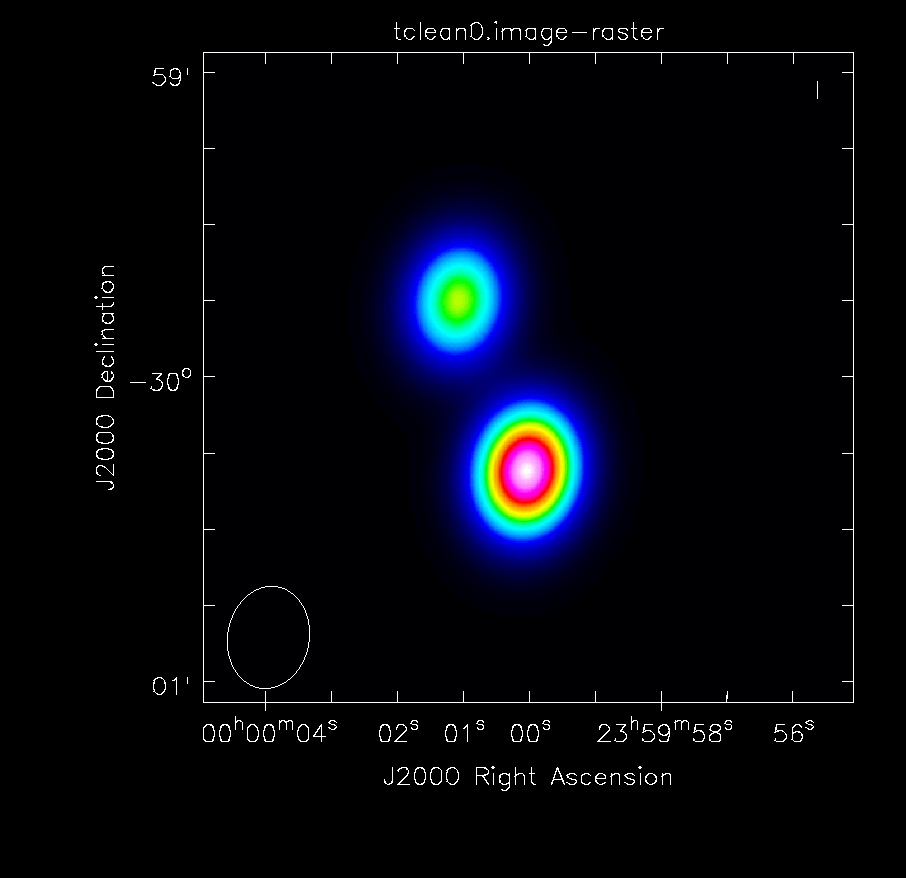
\includegraphics[height=3cm]{./chapters/01.intro/first.png}%
			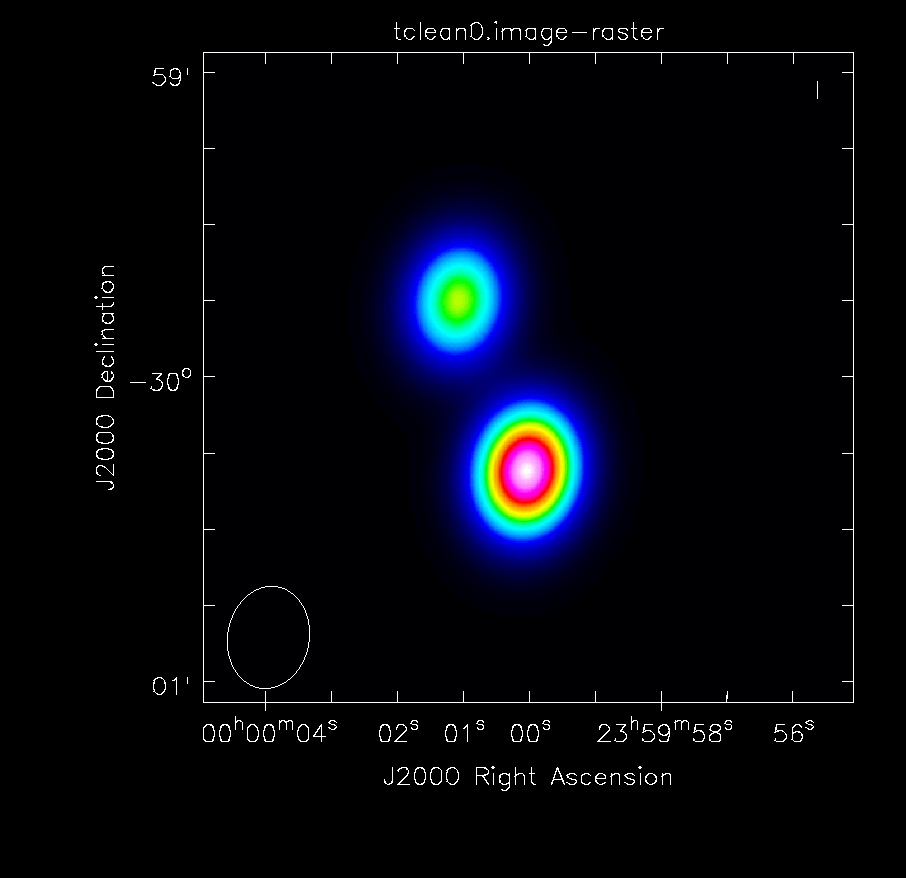
\includegraphics[height=3cm]{./chapters/01.intro/first.png}%
		}%
	}
	\setlength{\twosubht}{\ht\twosubbox}
	
	% typeset
	\centering
	\subcaptionbox{Measurements of the interferometer in the Fourier space.\label{intro0:inversefig:uvspace}}{%
		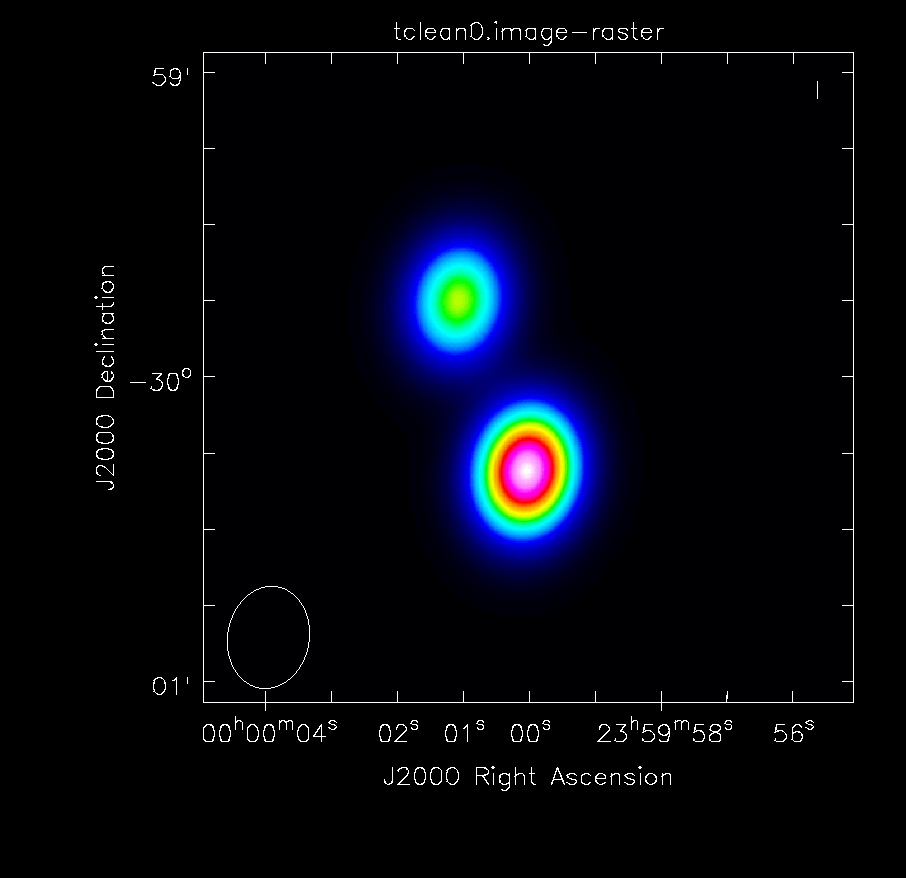
\includegraphics[height=\twosubht]{./chapters/01.intro/first.png}%
	}\quad
	\subcaptionbox{Observed image of the sky, showing two stars.\label{intro0:inversefig:reconstruction}}{%
		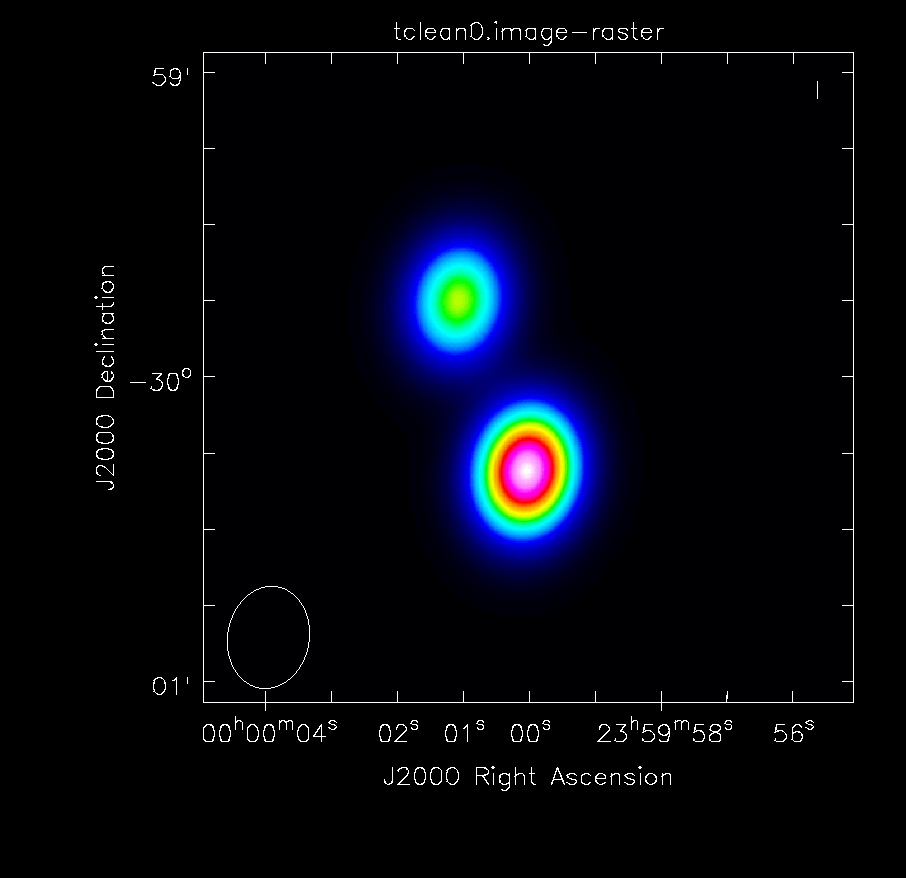
\includegraphics[height=\twosubht]{./chapters/01.intro/first.png}%
	}
	\caption{The image reconstruction problem, the observed image has to be reconstructed from the Fourier measurements.}\label{intro0:inversefig}
\end{figure}

At first glance, we might believe that the image reconstruction is trivial: The interferometer measures Fourier components, and efficient algorithms for the inverse Fourier transforms are well-known. However, two properties of the measured Fourier components make the image reconstruction difficult: The measurements are both noisy and incomplete.

The atmosphere of the earth is one source that introduces noise. It adds noise to the amplitude and phase of each measured Fourier component. The atmosphere changes over time and can under the right circumstances introduce a high level of noise compared to the signal. The image reconstruction should be able to find the observed image from potentially very noisy Fourier measurements.

The interferometer measures an incomplete set of Fourier components. Note that the Figure \ref{intro0:inversefig:uvspace} shows the Fourier space, which has missing components. The interferometer can only measure a limited set of Fourier components. The reconstruction algorithm has to find the observed image even though important Fourier components are missing from the measurements.

These two difficulties, the noise and the incomplete measurements, lead to the fact that there are many different candidate images that fit the measurements.  This is known as an inverse problem. We want to find the observed image, even though all we have are imperfect measurements. From the measurements alone, we cannot decide which candidate is the truly observed image. However, we have additional knowledge that simplifies the inverse problem: We know it is an image of the sky, which consists of stars, hydrogen clouds, etc. By including prior knowledge in the reconstruction, we can find the most likely image given the measurements. 

The question remains is: How close is the most likely image to the observed one? Is exact reconstruction possible where the most likely and observed image are equal? Surprisingly the answer is yes. It is possible in theory\cite{candes2006robust,donoho2006compressed}, and was shown in practice on low noise measurements\cite{dabbech2018cygnus, dabbech2015moresane}. However, not all algorithms perform equally well when the noise level in the measurements is high. Also, computing resources required for each algorithm can vary significantly. In short, a reconstruction algorithm has three opposing goals:
\begin{enumerate}
	\item Produce a reconstruction which is as close to the truly observed image as possible.
	\item Robust against even heavy noise in the measurements.
	\item Use as few computing resources as possible.
\end{enumerate}

No reconstruction algorithm performs equally well on all three goals. One of the most widely used reconstruction algorithms is CLEAN \cite{hogbom1974aperture, rau2011multi}. It has shown to be robust against heavy noise and, depending on the observation and is one of the oldest algorithms still in use today. As such, it was developed before the advent of distributed and GPU-accelerated computing. Today's new radio interferometers produce ever more measurements. The recently finished MeerKAT radio interferometer produces roughly 80 million Fourier measurements each second. Astronomers wish to reconstruct an image from several hours worth of measurement data. Reconstructing an image from this data volume requires GPU and distributed computation. But how to use GPU and distributed computing effectively is still an open problem.

Coordinate descent methods have been successfully applied in other inverse problems, such as reconstruction of CT scans\cite{bouman1996unified}, or X-Ray imaging\cite{felix2017compressed}. GPU accelerated\cite{mcgaffin2015edge} and distributed\cite{fercoq2014fast} variants have been developed. To our knowledge, coordinate descent methods have not been explored for the inverse problem in Radio Astronomy.

In this work, we develop our own proof-of-concept image reconstruction algorithm based on coordinate descent methods. We apply the reconstruction on a real world MeerKAT observation provided by SARAO. We explore the possible speedups we can achieve by using GPU and distributed computation. The algorithm is implemented platform independent in .netcore.

The rest of this work is structured as follows. First in section \ref{radio}, we give an introduction to radio interferometric imaging, and give the theoretical background to why a reconstruction can even achieve a higher resolution than the instrument. Next we present the current state-of-the-art in image reconstruction for radio interferometers in section \ref{state}. Then we derive a basic image reconstruction algorithm based on coordinate descent in section \ref{cd}, and show how we can use GPU acceleration and distribution to speed up reconstruction.

